%%%%%%%%%%%%%%%%%%%%%
%   AMS packages    %
%%%%%%%%%%%%%%%%%%%%%
\documentclass{beamer}
\usepackage{amsmath}
\usepackage{amsxtra}
\usepackage{amscd}
\usepackage{amsthm}
\usepackage{amsfonts}
\usepackage{amssymb}
\usepackage{eucal}
%\usepackage[all]{xy}
\usepackage{graphicx}
\usepackage{comment}
\usepackage{amssymb}
\usepackage{latexsym,amsmath,amscd,amssymb,epsfig,verbatim}
\usepackage{tikz}
\usetikzlibrary{arrows,shapes}
\usepackage{tikz-qtree}
\tikzset{level distance=50pt,
    sibling distance=7pt,
    every tree node/.style={align=center},}

\newtheorem{thm}{Theorem}
\newtheorem{cor}[thm]{Corollary}
\newtheorem{lem}[thm]{Lemma}
\newtheorem{prop}[thm]{Proposition}
\newtheorem{ex}[thm]{Exercise}
\newtheorem{conjecture}{Conjecture}
%\newtheorem*{conjecture*}{Conjecture}

\theoremstyle{remark}
\newtheorem{rem}[thm]{Remark}
\newtheorem{eg}[thm]{Example}

%\newtheorem{counterexample}[thm]{Counterexample}
\newtheorem{defn}[thm]{Definition}
%\newtheorem{claim}[thm]{Claim}
%\newtheorem{note}[thm]{Notation}
%\newtheorem{warning}[thm]{Warning}
%\newtheorem{variant}[thm]{Variant}
%\newtheorem{question}[thm]{Question}
%\newtheorem{construction}[thm]{Construction}
%\newtheorem{terminology}[thm]{Terminology}
%\newtheorem{convention}[thm]{Convention}

\newcommand\nc{\newcommand}
\nc\on{\operatorname}
\nc\renc{\renewcommand}
\newcommand\ssec{\subsection}
\newcommand\sssec{\subsubsection}
\newcommand\bO{{\mathbf O}}
\newcommand\CC{{\mathcal C}}
\newcommand\BN{{\mathbb N}}
\newcommand\BC{{\mathbb C}}
\newcommand\BF{{\mathbb F}}
\newcommand\BR{{\mathbb R}}
\newcommand\BQ{{\mathbb Q}}
\newcommand\BBZ{{\mathbb Z}}
\newcommand\uR{\underline{R}}
\newcommand\uZ{\underline{\BBZ}}
\newcommand\CF{{\mathcal F}}
\newcommand\uCF{\underline{{\mathcal F}}}
\newcommand\BZ{{\mathbb Z}}
\newcommand\BA{{\mathbb A}}
\newcommand\BP{{\mathbb P}}
\newcommand\fa{{\mathfrak a}}
\newcommand\fp{{\mathfrak p}}
\newcommand\fq{{\mathfrak q}}
\newcommand\fm{{\mathfrak m}}
\newcommand\pt{\mathrm{pt}}
\newcommand\rk{\operatorname{rk}}
\newcommand\Aut{\operatorname{Aut}}




\newcommand\fbn{\mathcal H}
\newcommand \edgequot{\text{edge-quotient bijective }}

\def\Stab{\operatorname{Stab}}
\def\Fix{\operatorname{Fix}}
\newcommand\im{\text{Im}}

\newcommand\Wider[2][3em]{%
\makebox[\linewidth][c]{%
  \begin{minipage}{\dimexpr\textwidth+#1\relax}
  \raggedright#2
  \end{minipage}%
  }%
}


% \AtBeginSection[]{
% 	\begin{frame}{Outline of Talk}
% 		\tableofcontents[currentsection]
% 	\end{frame}
% }

\mode<presentation>{}
\usetheme{Frankfurt}
\usecolortheme{seahorse}

%%%%%%%%%%%%   Title slide info  %%%%%%%%%%%%%
\title{Peckness of Edge Posets}
\author{David Hemminger*\inst{1}, Aaron Landesman\inst{2}, Zijian Yao\inst{3}}
 
\institute[VFU] % (optional)
{
  \inst{1}
  Duke University
,
  \inst{2}
  Harvard University
  ,
  \inst{3}
  Brown University
}

\begin{document}

%%%%%%%%%%%%  Title Frame  %%%%%%%%%%%%%%%%
\begin{frame}
	\titlepage
\end{frame}


%%%%%%%%%%%% Talk Outline %%%%%%%%%%%%%%%%%%%
% \begin{frame}{Outline of Talk}
% 	\tableofcontents
% \end{frame}






%%%%%%%%%%%%%%%%%%%%   Background Section   %%%%%%%%%%%%%%%%%%%

\section{Background}
\subsection{}




\begin{frame}{Basic Definitions}

\begin{defn}
Let $P$ be a finite graded poset of rank $n$. That is:
\begin{itemize}
\item Elements of $P$ are a disjoint union of $P_0,P_1,\ldots,P_n$, called the \textit{ranks}
\item If $x\in P_i$ and $x\lessdot y$, then $y\in P_{i+1}$
\item Define $\rk(x) = k$, where $x\in P_k$.
\end{itemize}
\end{defn}

% \begin{defn}
% A map $f\colon P\rightarrow Q$ is a \textit{morphism} from $P$ to $Q$ if $x\le_P y \implies f(x)\le_Q f(y)$ and $\rk(x) = \rk(f(x))$.  We say that $f$ is \textit{injective/surjective/bijective} if it is an injection/surjection/bijection from $P$ to $Q$ as sets.
% \end{defn}
\end{frame}









\begin{frame}{Peck Posets}
\begin{defn}
Write $p_i = |P_i|$.  P is
\begin{itemize}

\item \textit{Rank-symmetric} if $p_i = p_{n-i}$ for all $1\le i\le n$

\item \textit{Rank-unimodal} if for some $0\le k\le n$ we have
$$p_0\le p_1\le \ldots \le p_k \ge p_{k+1} \ge\ldots \ge p_n$$

\item \textit{$k$-Sperner} if no union of $k$ antichains (sets of pairwise incomparable elements) in $P$ is larger than the union of the largest $k$ ranks of $P$

\item \textit{Strongly Sperner} if it is $k$-Sperner for all $1\le k\le n$.

\item \textit{Peck} if $P$ is rank-symmetric, rank-unimodal, and strongly Sperner.
\end{itemize}
\end{defn}
\end{frame}







% \begin{frame}

% \begin{defn}
% Let $V(P)$ and $V(P_i)$ be the complex vector spaces with bases $\{x |x\in P\}$ and $\{x |x\in P_i\}$
% \end{defn}

% \begin{lem}[Stanley, 1982]
% $P$ is Peck if and only if there exists an linear transformation $U\colon V(P)\rightarrow V(P)$ such that
% \begin{itemize}
% \item For every basis element $x\in P$, 
% $$U(x) = \sum_{y\gtrdot x} c_{x,y}y$$

% \item  For all $0\le i < \frac{n}{2}$, the map $U^{n-2i}\colon V(P_i)\rightarrow V(P_{n-i})$ is an isomorphism.
% \end{itemize}
% \end{lem}
% \end{frame}







% \begin{frame}
% \begin{defn}
% If the Lefschetz map defined by

% $$L(x) = \sum_{y\gtrdot x} y$$

% satisfies the second condition in the previous lemma, then $P$ is \textit{unitary Peck}.
% \end{defn}
% \end{frame}






%%%%%%%%%%%%%%%%%%%%   Edge Poset    %%%%%%%%%%%%%%%%%%%


\section{Edge Poset Construction and Main Result}
\subsection{}

\begin{frame}{Definition of the Edge Poset}
\begin{defn}
\label{defn:functor_of_edges}
For $P$ a finite graded poset, its \textit{edge poset} $\mathcal{E}(P)$ is the finite graded poset defined as follows. 
\begin{itemize}

\item Elements of $\mathcal{E}(P)$ are ordered pairs $(x,y)\in P\times P$ where $x\lessdot y$

\item Define $(x,y) \lessdot_{\mathcal{E}} (x^\prime,y^\prime)$ if $x\lessdot_P x^\prime$ and $y\lessdot_P y^\prime$

\item Define $\le_{\mathcal{E}}$ to be the transitive closure of $\lessdot_{\mathcal{E}}$

\item Define $\rk_{\mathcal{E}}(x,y) = \rk_P(x)$.
\end{itemize}
\end{defn}
\end{frame}










\begin{frame}{Basic Example}
\begin{center}
\begin{tikzpicture}[scale=.5] at (0,0)
  \node (0) at (0,0) {$0$};
  \node (1) at (-1,2) {$1$};
  \node (2) at (1,2) {$2$};
  \node (3) at (0,4) {$3$};
  \node (4) at (2,4) {$4$};
  \node (5) at (0,6) {$5$};
  \node (6) at (2,6) {$6$};
  \node (7) at (1,8) {$7$};
  \draw (0)--(1);
  \draw (0)--(2);
  \draw (1)--(3);
  \draw (2)--(3);
  \draw (2)--(4);
  \draw (3)--(5);
  \draw (4)--(6);
  \draw (5)--(7);
  \draw (6)--(7);
  \node (8) at (0,-2) {$P$};
\end{tikzpicture} \qquad
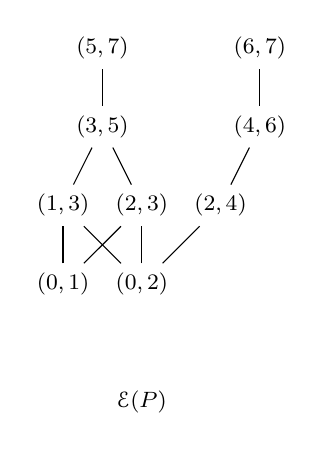
\begin{tikzpicture}[scale = .5]
  \node[font=\footnotesize] (0) at (0,1) {$(0,1)$};
  \node[font=\footnotesize] (1) at (2,1) {$(0,2)$};
  \node[font=\footnotesize] (2) at (0,3) {$(1,3)$};
  \node[font=\footnotesize] (3) at (2,3) {$(2,3)$};
  \node[font=\footnotesize] (4) at (4,3) {$(2,4)$};
  \node[font=\footnotesize] (5) at (1,5) {$(3,5)$};
  \node[font=\footnotesize] (6) at (5,5) {$(4,6)$};
  \node[font=\footnotesize] (7) at (1,7) {$(5,7)$};
  \node[font=\footnotesize] (8) at (5,7) {$(6,7)$};
  \draw (0)--(2);
  \draw (0)--(3);
  \draw (1)--(2);
  \draw (1)--(3);
  \draw (1)--(4);
  \draw (2)--(5);
  \draw (3)--(5);
  \draw (4)--(6);
  \draw (5)--(7);
  \draw (6)--(8);
  \node[font=\footnotesize] (9) at (2,-2) {$\mathcal E(P)$};
\end{tikzpicture} 
\end{center}
\end{frame}












\begin{frame}{Conjecture on the Peckness of Edge Posets}
\begin{defn}
The \textit{boolean algebra of rank $n$}, denoted $B_n$, is the poset whose elements are subsets of $[n]$ with order given by containment, i.e. for $x,y\in B_n$, $x\le y$ if $x\subseteq y$.
\end{defn}

\begin{conjecture}[Hemminger, Landesman, and Yao 2014]
Let $G\subseteq \Aut(B_n)$.  Then $\mathcal{E}(B_n/G)$ is Peck.
\end{conjecture}
\end{frame}








%%%%%%%%%%%%%%%%%%%%   Main Result    %%%%%%%%%%%%%%%%%%%

%\section{Main Result}
\subsection{}

\begin{frame}{Main Result}
\begin{defn}
A group action of $G$ on $P$ is \textit{common cover transitive} (CCT) if whenever $x,y,z\in P$ such that $x\lessdot z$, $y\lessdot z$, and $y\in Gx$, there exists some $g\in \Stab_G(z)$ such that $g\cdot x = y$.
\end{defn}

\begin{thm}[Hemminger, Landesman, and Yao 2014]
If a group action of $G$ on $B_n$ is CCT, then $\mathcal{E}(B_n/G)$ is Peck.
\end{thm}
\end{frame}








% \begin{frame}
% \begin{defn}
% Given a group action of $G$ on $P$, define a group action of $G$ on $\mathcal{E}(P)$ by letting $g\cdot (x,y) = (g\cdot x,g\cdot y)$ for all $g\in G$.
% \end{defn}
% \pause
% \begin{prop}
% The map $q\colon \mathcal{E}(P)/G\rightarrow \mathcal{E}(P/G)$ defined by $q(G(x,y)) = (Gx,Gy)$ is a surjective morphism.  Furthermore, $q$ is also injective if and only if the action of $G$ on $P$ is CCT.
% \end{prop}

% \begin{lem}
% If $f:P\rightarrow Q$ is a bijective morphism and $P$ is Peck then $Q$ is Peck.
% \end{lem}
% \end{frame}









% \begin{frame}
% \begin{thm}[Stanley, 1984; Harper, 1984; Pouzet and Rosenberg, 1986]
% If $P$ is unitary Peck and $G\subseteq\operatorname{Aut}(P)$, then $P/G$ is Peck.
% \end{thm}
% It suffices to show that $\mathcal{E}(B_n)$ is unitary Peck. Our proof of this is complicated. Instead, we construct a unitary Peck poset $\mathcal{H}(B_n)$ such that there is a bijective morphism $\mathcal{H}(B_n)/G\rightarrow \mathcal{E}(B_n)/G$.

% \end{frame}








% \begin{frame}{Definition of $\mathcal{H}(P)$}
% \begin{defn}

% For $P$ a finite graded poset, define the graded poset $\mathcal H(P)$ as follows.
% \begin{itemize}
% \item Elements are pairs $(x,y)\in P\times P$ such that $x\lessdot y$

% \item Define $(x,y) \lessdot_{\mathcal H} (x^\prime,y^\prime)$ if $x \lessdot_P x^\prime,y\lessdot_P y^\prime$ \textbf{and} $\mathbf{y \ne x^\prime}$

% \item Define $\leq_{\mathcal H}$ to be the transitive closure of $\lessdot_{\mathcal H}$

% \item Define $rk_{\mathcal H}(x,y) = rk_P(x).$

% \end{itemize}
% \end{defn}
% \end{frame}






% \begin{frame}{The Boolean Algebra $B_3$}

% \begin{figure}
% \centering
% \begin{tikzpicture}[scale = 1.7]
%   \node (0) at (0,0) {$\emptyset$};
%   \node (1) at (-1,1) {$\{1\}$};
%   \node (2) at (0,1) {$\{2\}$};
%   \node (3) at (1,1) {$\{3\}$};
%   \node (4) at (-1,2) {$\{1,2\}$};
%   \node (5) at (0,2) {$\{1,3\}$};
%   \node (6) at (1,2) {$\{2,3\}$};
%   \node (7) at (0,3) {$\{1,2,3\}$};
%   \draw (0)--(1);
%   \draw (0)--(2);
%   \draw (0)--(3);
%   \draw (1)--(4);
%   \draw (1)--(5);
%   \draw (2)--(4);
%   \draw (2)--(6);
%   \draw (3)--(5);
%   \draw (3)--(6);
%   \draw (4)--(7);
%   \draw (5)--(7);
%   \draw (6)--(7);
%   \node (9) at (0,-.5) {$B_3$};
% \end{tikzpicture}
% \end{figure}
% \end{frame}






% \begin{frame}{$\mathcal{H}(B_3)$ is unitary Peck}
% \Wider{
% \begin{figure}
% \centering
% \begin{tikzpicture}[scale = 1]
% \tikzstyle{every node}=[font=\small]
%   \node (0) at (0,0) {$(\emptyset,\{1\})$};
%   \node (1) at (4,0) {$(\emptyset,\{2\})$};
%   \node (2) at (8,0) {$(\emptyset,\{3\})$};
%   \node (3) at (3,1) {$(\{1\},\{1,2\})$};
%   \node (4) at (7,1) {$(\{1\},\{1,3\})$};
%   \node (5) at (-1,1) {$(\{2\},\{1,2\})$};
%   \node (6) at (9,1) {$(\{2\},\{2,3\})$};
%   \node (7) at (1,1) {$(\{3\},\{1,3\})$};
%   \node (8) at (5,1) {$(\{3\},\{2,3\})$};
%   \node (9) at (8,2) {$(\{1,2\},\{1,2,3\})$};
%   \node (10) at (4,2) {$(\{1,3\},\{1,2,3\})$};
%   \node (11) at (0,2) {$(\{2,3\},\{1,2,3\})$};
%   \draw (0)--(5)--(11)--(7)--(0);
%   \draw (1)--(3)--(10)--(8)--(1);
%   \draw (2)--(4)--(9)--(6)--(2);
%   \node (9) at (4,-1) {$\mathcal H(B_3)$};
% \end{tikzpicture}
% \end{figure}
% }

% \end{frame}





% \begin{frame}
% \begin{defn}
% As before, for $G$ acting on $\mathcal H(P)$, define $g\cdot (x,y) = (g\cdot x,g\cdot y)$.
% \end{defn}

% \begin{rem}
% Since $\mathcal{E}(P)$ and $\mathcal{H}(P)$ have the same elements and $(x,y)\le_{\mathcal{H}} (x^\prime,y^\prime) \implies (x,y)\le_{\mathcal{E}} (x^\prime,y^\prime)$, there is a natural bijective morphism $\mathcal{H}(P)/G\rightarrow \mathcal{E}(P)/G$.
% \end{rem}

% \begin{proof}[Proof of Main Result]
% $\mathcal{H}(B_n)$ unitary Peck $\implies \mathcal{H}(B_n)/G$ Peck $\implies \mathcal{E}(B_n)/G$ Peck $\implies \mathcal{E}(B_n/G)$ Peck.
% \end{proof}
% \end{frame}








%%%%%%%%%%%%%%%%%%%%   CCT Actions    %%%%%%%%%%%%%%%%%%%

\section{CCT Actions}
\subsection{}

% \begin{frame}{CCT actions}
% \begin{lem}
% \label{lem:cover_transitive_equivalence}
% Let $G$ be a group acting on a graded poset $P.$ The following are equivalent:
% \begin{enumerate}
% 	\item The action of $G$ on $P$ is CCT.
% 	\item Whenever $w \lessdot x,w \lessdot y,$ and $x \in Gy,$ there exists some $g \in Stab(w)$ with $gx = y.$
% 	\item The map $q\colon \mathcal E(P)/G\rightarrow \mathcal E(P/G)$ defined by $q(G(x, z)) = (Gx,Gz)$ is a bijective morphism (but not necessarily an isomorphism).
% 	\item For all $i$ there is an equality $|(\mathcal E(P)/G)_i|=| (\mathcal E(P/G))_i|$
% \end{enumerate}
% \end{lem}
% \end{frame}





\begin{frame}{Some examples of CCT actions}
\begin{block}{CCT Actions}
\begin{enumerate}
\item The trivial group;
\pause
\item The group $S_n$ acting on $B_n$;
\pause
\item The group $D_{2n}$ acting on $B_{n}$ when $n = p$ or $n = 2p$, and $p$ is a prime;
\pause
\item The elementary $2$-group $(\mathbb Z /2 \mathbb Z)^k$ with any action on $B_n$.
\end{enumerate}
\end{block}
\end{frame}





\begin{frame}{The direct product and semi-direct product}
\begin{lem}
\label{thm:direct_product_preservation}
For $\phi:G\times P\rightarrow P,\psi:H \times Q \rightarrow Q$ two CCT actions, then the direct product $\phi \times \psi:(G\times H)\times (P\times Q) \rightarrow (P\times Q),(g,h)\cdot (x,y) \mapsto (gx,hy)$ is also CCT.
\end{lem}
%\end{frame}





%\begin{frame}{The semi-direct product}
\begin{prop}\label{prop:semidirect_product_cover_transitive_actions}
Let $G\subseteq \operatorname{Aut}(P)$, $H\triangleleft G$, $K\subset G$ such that $G = H\rtimes K$.  Suppose that the action of $H$ on $P$ is CCT and the action of $K$ on $P/H$ is CCT.  Then the action of $G$ on $P$ is CCT.
\end{prop}
\end{frame}





\begin{frame}{The wreath product}
\begin{cor}
\label{thm:wreath_preservation}
If $\psi:G\times P \rightarrow P$ is CCT, then $\phi:G\wr S_l \times P^l \rightarrow P^l$ where $\phi$ is the induced action is also CCT.
\end{cor}
\pause
\begin{cor}
The action $S_m \wr S_l \times B_{n} \rightarrow B_{n}$ is CCT, where $n =ml$.
\end{cor}
\pause
\begin{rem}
This recovers a special case of \cite[Theorem 1.1]{pak}: 

The poset $\mathcal E (B_n/S_m \wr S_l)$ is rank symmetric and rank unimodal. (Furthermore, it is Peck!)
\end{rem}
\end{frame}





% \begin{frame}{The automorphism of rooted trees}
% \begin{center}
% \Tree [.root [.$\bullet$  1 2 ] [.$\bullet$  3 4 ] [.$\bullet$  [.$\bullet$  5 6 7 ] [.$\bullet$  8 9 10 ] ] [.$\bullet$  11  12 ] ]
% \end{center}
% \end{frame}





% \begin{frame}{Automorphism of rooted trees}
% \begin{prop}
% Let $P$ be a rooted tree. Then, 
% $$Aut(P) = (G_1 \wr S_{i_1}) \times (G_2 \wr S_{i_2}) \times \cdots \times (G_m\wr S_{i_m}),$$
% \end{prop}
% \pause
% \begin{cor}
% Let $P$ be a rooted tree with leaves $L(P)$, and let $n = |L(P)|$, then the action of $Aut(P)$ on $B_n$  induced  from the action of $Aut(P)$ on $L(P)$  is CCT. 
% \end{cor}
% \end{frame}





% \begin{frame}{Rooted trees and the wreath product}
% \begin{center}
% \Tree [.root [.$\bullet$  1 2 3 4 ]  [.$\bullet$  5 6 7 8 ]  [.$\bullet$  9 10 11 12 ]  ]
% \end{center}
% \end{frame}









%%%%%%%%%%%%%%%%%%%%   Non-CCT Actions   %%%%%%%%%%%%%%%%%%%

% \section{Non-CCT actions}
% \subsection{}

% \begin{frame}{Unimodality of ranks of certain edge posets}
% \begin{lem}
% Let $C_n$ be the cyclic group which acts naturally on $B_n$, then size of the $i^{th}$ rank of the poset $\mathcal E (B_n)/C_n$ is $$|\mathcal E (B_n)/C_n|_{i} = \binom{n-1}{i}.$$
% \end{lem}
% \pause
% \begin{lem}
% Let $C_p$ be the cyclic group with prime order $p$, then  $$|(\mathcal E (B_p)/C_p)_i| - |\mathcal E(B_p/C_p)_i| = \frac{p-1}{2}.$$
% \end{lem}
% \pause
% \begin{prop}
% The poset $\mathcal E (B_n/C_n)$ is rank symmetric and rank unimodal.
% \end{prop}
% \end{frame}






% \begin{frame}{Unimodality of ranks of certain edge posets}
% \begin{lem}
% Let $D_{2n}$ be the dihedral group of size $2n$ which acts naturally on $B_n$, then size of the $i^{th}$ rank of the poset $\mathcal E (B_n)/D_{2n}$ is
% $$|\mathcal E (B_n)/D_{2n}|_{i}  = \frac{1}{2} \Big( {n-1 \choose i } + \frac{1}{2} [(-1)^{n(i+1)}+1] \cdot { \lceil n/2\rceil -1  \choose \lceil (i+1)/2 \rceil - 1}  \Big)$$
% \end{lem}
% \pause
% \begin{prop}
% The poset $\mathcal E (B_n/D_{2n})$ is rank symmetric and rank unimodal.
% \end{prop}
% \end{frame}





% %%%%%%%%%%%%%%%%   q - analog and higher r   %%%%%%%%%%%%%%%%%%

% \section{Final remarks}
% \subsection{}

% \begin{frame}{The $q$ analog of the problem}
% \begin{block}{The $q$-Boolean algebra}
% Let $B_n(q)$ be the poset of all $\mathbb F_q$-subspaces of $V_n(q) := (\mathbb F_q)^n$, and $G < Gl_n(\mathbb F_q)$. We consider $\mathcal E (B_n(q))/G$ and $\mathcal E(B_n(q)/G)$.
% \end{block}
% \pause
% \begin{lem} 
% Let $q$ be a prime,  then $$ |\mathcal F^1 \big(B_n(q)\big)/C_n(q)|_{i} = {n-1 \choose i}_q.$$
% \end{lem}
% \pause
% \begin{block}{Questions}
%  Is $\mathcal E \big(B_n(q) /G\big)$ Peck? or more weakly, is it rank unimodal?
% \end{block}
% \end{frame}






% \begin{frame}{Some Generalizations of $\mathcal{E}$ and Remarks}

% \begin{block}{$\mathcal E^r(P)$}
% Similarly we can define the $\mathcal E^r (P)$ on a graded poset $P$. The elements of $\mathcal E^r(P)$ are $(x, y)$ where $x,y\in P$, $x\le_P y$, and $\rk(y) = \rk(x) + r$. Define the covering relation $\lessdot_{\mathcal E}$ by $(x, y) \lessdot_{\mathcal E} (x^\prime, y^\prime)$ if $x\lessdot_P x^\prime$ and $y\lessdot_P y^\prime$.  
% \end{block}
% \pause
% \begin{block}{Other generalizations}
% $\mathcal H^r(P)$; \quad  $\mathcal E^{\vec{r}} (P)$; \quad $\mathcal H^{\vec{r}} (P). $
% \end{block}
% \end{frame}



\section{Acknowledgements}
\subsection{}

\begin{frame}{References}
\nocite{quotients_stanley}
\nocite{algebraic_stanley}
\nocite{pak}
\bibliography{References}
\bibliographystyle{alpha}
\end{frame}


\begin{frame}{Acknowledgements}
\begin{enumerate}
\item Thanks to Dr. Vic Reiner and Elise DelMas for mentoring and TAing this project. We also thank Ka Yu Tam for helpful comments. 
\item The work for this project took place at the Minnesota at Twin Cities REU.  Thanks to Dr. Gregg Musiker and the University of Minnesota School of Mathematics for coordinating and hosting the REU.
\item This research was supported by the RTG grant NSF/DMS-1148634.
\end{enumerate}
\end{frame}

\end{document}





